\begin{surferIntroPage}{SURFER 시작하기}{tutorial_koord1}{SURFER 시작하기}
이 프로그램은 SURFER 라고 합니다. 이 단어를 보면 아마 여러분은 물, 태양 그리고 파도를 떠올릴 지도 모릅니다. 하지만 이 단어는 {\it surface} 라는 단어에서 유래하였습니다.
\\
SURFER를 이용하여 우리는 곡면(surface), 더 정확하게는 대수곡면을 표현할 수 있습니다. 
이 튜토리얼에는 대수곡면의 성질과 SURFER의 사용법이 설명되어 있습니다.\\
SURFER는 2008 독일 수학의 해에 시작된 이동 전시 프로젝트인 IMAGINARY의 프로그램 중 하나입니다. IMAGINARY는 독일 남서부 삼림지대 오버볼파크에 있는 수학연구소(Mathematisches Forschungsinstitut Oberwolfach)에 의해 기획되었습니다. 연구소에서는 매주 최신 수학을 주제로 워크숍이 열립니다. 이 워크숍은 전세계 수학자의 교류를 활성화 시키는 데에 굉장히 중요한 역할을 합니다.\\
\vspace{0.2cm} \hspace{3.5cm}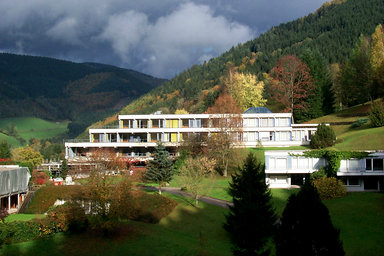
\includegraphics[width=3cm]{./../../common/images/photo_mfo.jpg}\\
이 프로그램은 다음의 웹사이트에서 다운받을 수 있습니다.: \\
\begin{centering}
www.imaginary.org\\
\end{centering}
 \vspace{0.2cm}
오른쪽에서 여러분은 레몬부터 시작하는 수학 튜토리얼을 선택할 수 있습니다. 왼쪽에서는 환상적인 곡면들 같은 다른 갤러리로 이동할 수 있습니다.
\end{surferIntroPage}
